\documentclass[11pt]{article}

\usepackage[margin=1in]{geometry}
\usepackage[T1]{fontenc}
\usepackage{lmodern}
\usepackage{microtype}
\usepackage{graphicx}
\usepackage{booktabs}
\usepackage{longtable}
\usepackage{array}
\usepackage{xcolor}
\usepackage{hyperref}
\usepackage{enumitem}
\usepackage{listings}
\usepackage{tikz}
\usetikzlibrary{arrows.meta,positioning,shapes.geometric,shapes.multipart,fit,calc}

\hypersetup{
  colorlinks=true,
  linkcolor=blue,
  urlcolor=blue,
  citecolor=blue,
  pdftitle={dont-be-square: FAIR Score Visualizer for HuBMAP Datasets},
  pdfauthor={Project report (auto-generated)},
}

\definecolor{codebg}{RGB}{248,248,248}
\definecolor{codeframe}{RGB}{220,220,220}
\definecolor{darkgray}{RGB}{60,60,60}

\lstdefinestyle{base}{
  basicstyle=\ttfamily\small,
  backgroundcolor=\color{codebg},
  frame=single,
  rulecolor=\color{codeframe},
  columns=fullflexible,
  keepspaces=true,
  showstringspaces=false,
  breaklines=true,
  upquote=true,
}

\lstdefinestyle{python}{
  style=base,
  language=Python,
  keywordstyle=\color{blue!70!black},
  stringstyle=\color{green!40!black},
  commentstyle=\color{darkgray},
}

\lstdefinestyle{xml}{
  style=base,
  language=XML,
  keywordstyle=\color{blue!70!black},
  stringstyle=\color{green!40!black},
  commentstyle=\color{darkgray},
}

\title{\textbf{dont-be-square}\\FAIR Score Visualizer for HuBMAP Datasets\\\large Technical Report}
\author{Generated from repository source analysis}
\date{\today}

\begin{document}
\maketitle
\tableofcontents
\newpage

\section{Executive Summary}
The \texttt{dont-be-square} project computes a \textbf{FAIR score}---\textit{Findable}, \textit{Accessible}, \textit{Interoperable}, and \textit{Reproducible}---for HuBMAP datasets identified by a \texttt{hubmap\_id} (e.g., \texttt{HBM666.NDQZ.365}). It provides two user-facing paths:
\begin{itemize}[leftmargin=2em]
  \item \textbf{Live scoring (single dataset)}: a Streamlit app where a user enters a HuBMAP dataset ID, the app fetches metadata from HuBMAP APIs, runs the four scoring modules, and renders a 2$\times$2 heatmap image.
  \item \textbf{Batch precompute + explore}: a batch script discovers many datasets (via HuBMAP Search and Entity APIs), computes FAIR results, stores them in \texttt{fair/fair\_results.json}, and a second Streamlit app loads that JSON to filter/aggregate scores by lab (group), assay type, or specific dataset.
\end{itemize}

\section{Repository Structure}
Key files and responsibilities are summarized in Table~\ref{tab:structure}.

\begin{longtable}{@{}p{0.32\textwidth}p{0.62\textwidth}@{}}
\caption{Important files and modules in the repository.}\label{tab:structure}\\
\toprule
\textbf{Path} & \textbf{Purpose} \\
\midrule
\endfirsthead
\toprule
\textbf{Path} & \textbf{Purpose} \\
\midrule
\endhead
\bottomrule
\endfoot
\texttt{streamlit\_app.py} & Live scoring UI: user inputs a single \texttt{hubmap\_id}, calculates FAIR scores, saves/displays a heatmap PNG. \\
\texttt{streamlit\_test.py} & ``Explore'' UI: loads precomputed \texttt{fair/fair\_results.json}; filter by Lab / Assay / Lab+Assay / ID / All; computes mean FAIR and plots heatmap. \\
\texttt{create\_fair\_json.py} & Batch pipeline: discover datasets by lab (group\_name) using HuBMAP Search API; fetch entities; compute FAIR scores for each dataset; write \texttt{fair/fair\_results.json}. \\
\texttt{fair/} & Core scoring package: \texttt{findable.py}, \texttt{accessible.py}, \texttt{interoperable.py}, \texttt{reproducible.py}, and utility code in \texttt{utils.py}. \\
\texttt{fairhelp.py} & Visualization: renders a 2$\times$2 heatmap using Matplotlib and saves a PNG. \\
\texttt{fair/fair\_results.json} & Precomputed results store (batch output) used by \texttt{streamlit\_test.py}. \\
\texttt{example.py} & Simple non-UI example of scoring + plotting on hardcoded dataset(s). \\
\texttt{testing\_utils.py} & Example script for searching/filtering in \texttt{fair\_results.json} and plotting aggregated results. \\
\end{longtable}

\section{Dependencies, Tools, and External Services}
\subsection{Core Python Libraries}
The project declares the following dependencies (see \texttt{requirements.txt}):

\begin{center}
\begin{tabular}{@{}p{0.28\textwidth}p{0.62\textwidth}@{}}
\toprule
\textbf{Library} & \textbf{Role in this project} \\
\midrule
\texttt{streamlit} & Web UI, inputs, status messages, progress bars, image display. \\
\texttt{requests} & HTTP calls to HuBMAP Entity API and validation endpoints (ORCID/UniProt/DOI). \\
\texttt{hubmap\_sdk} & Batch discovery and entity retrieval via HuBMAP Search/Entity APIs. \\
\texttt{pandas} & Loading/structuring precomputed JSON into DataFrames; filtering and aggregation. \\
\texttt{numpy} & Aggregations (means), reshaping to 2$\times$2 grids for plotting. \\
\texttt{matplotlib} & Rendering the FAIR heatmap PNG. \\
\texttt{tqdm} & Loop progress indicators (sometimes used with Streamlit UI). \\
\texttt{plotly}, \texttt{seaborn}, \texttt{humanize} & Listed as dependencies; minimal or no usage in the current code path. \\
\bottomrule
\end{tabular}
\end{center}

\subsection{External APIs and Data Sources}
The computation depends on multiple external services:
\begin{itemize}[leftmargin=2em]
  \item \textbf{HuBMAP Entity API}: primary source of dataset metadata used by all scoring modules.
  \item \textbf{HuBMAP Search API (via \texttt{hubmap\_sdk})}: used to discover dataset IDs by lab/group or other criteria for batch workflows.
  \item \textbf{ORCID API}: used to validate contributor/contact ORCID identifiers (Findable).
  \item \textbf{UniProt REST API}: used to validate antibody accession numbers (Findable).
  \item \textbf{DOI resolvers}: \texttt{doi.org} / \texttt{dx.doi.org} are used to check DOI link accessibility (Accessible).
\end{itemize}

\section{Data Model}
\subsection{Primary runtime object: \texttt{metadata} JSON}
All four FAIR pillars use a shared metadata-fetch function (implemented in \texttt{fair/findable.py}) that retrieves a JSON document from the HuBMAP Entity API. This metadata is treated as a Python \texttt{dict} and inspected for keys and values required by scoring rules.

\subsection{Precomputed storage: \texttt{fair/fair\_results.json}}
Batch computations are stored as JSON. A representative record (truncated) looks like:

\begin{lstlisting}[style=xml,caption={Representative structure of \texttt{fair/fair\_results.json} (schema illustration).}]
[
  [
    {
      "group_name": "University of California San Diego TMC",
      "hubmap_id": "HBM247.HLXR.494",
      "dataset_type": "RNAseq [Salmon]",
      "fair": [0.75, 0.42857142857142855, 0.5714285714285714, 1.0],
      "data_types": ["salmon_sn_rnaseq_10x"]
    }
  ],
  ...
]
\end{lstlisting}

\noindent\textbf{Observed schema properties:}
\begin{itemize}[leftmargin=2em]
  \item Top-level is a list where each element is itself a list (often length 1).
  \item Each inner list contains one or more objects with keys:
    \begin{itemize}
      \item \texttt{group\_name}: lab / consortium group name (string)
      \item \texttt{hubmap\_id}: dataset identifier (string)
      \item \texttt{dataset\_type}: dataset/assay type (string)
      \item \texttt{fair}: list of four floats \([F, A, I, R]\), each typically in \([0, 1]\)
      \item \texttt{data\_types}: list of strings (optional; sometimes \texttt{null})
    \end{itemize}
\end{itemize}

\section{System Workflows}
\subsection{Workflow A: Live scoring (single dataset) --- \texttt{streamlit\_app.py}}
\textbf{Goal:} interactive scoring of one dataset ID and immediate visualization.

\textbf{Steps:}
\begin{enumerate}[leftmargin=2em]
  \item User enters a \texttt{hubmap\_id}.
  \item On button click, the app calls the four scoring functions:
  \texttt{findable()}, \texttt{accessible()}, \texttt{interoperable()}, \texttt{reproducible()}.
  \item Each scoring function fetches metadata and evaluates a set of boolean checks (0/1).
  \item The module mean is computed as the pillar score.
  \item The app reshapes \([F, A, I, R]\) into a 2$\times$2 matrix and calls \texttt{fairhelp.create\_fair\_plot}.
  \item A PNG is saved locally and displayed in Streamlit.
\end{enumerate}

\subsection{Workflow B: Batch precompute + explore --- \texttt{create\_fair\_json.py} + \texttt{streamlit\_test.py}}
\textbf{Goal:} compute FAIR scores across many datasets and explore aggregate patterns.

\textbf{Batch precompute:}
\begin{enumerate}[leftmargin=2em]
  \item Use HuBMAP Search API to find datasets matching a lab/group (group\_name).
  \item Convert search hits into dataset entities using HuBMAP Entity API.
  \item Convert dataset objects into DataFrame rows.
  \item For each dataset row, compute the four pillar scores and store \texttt{fair=[F,A,I,R]}.
  \item Write to \texttt{fair/fair\_results.json}.
\end{enumerate}

\textbf{Explore UI:}
\begin{enumerate}[leftmargin=2em]
  \item Load \texttt{fair/fair\_results.json} into a DataFrame.
  \item Filter records by Lab / Assay / Lab+Assay / ID / All.
  \item Compute mean FAIR vector across the selected set.
  \item Render and display a heatmap for the aggregate scores.
\end{enumerate}

\section{FAIR Scoring Methodology (Module-by-Module)}
Each pillar produces:
\begin{itemize}[leftmargin=2em]
  \item \textbf{score}: a float computed as the mean of a list of checks (0/1 or booleans coerced to integers)
  \item \textbf{detail list}: the underlying per-check values (useful for debugging and transparency)
\end{itemize}

\subsection{Findable (\texttt{fair/findable.py})}
\textbf{Inputs:} \texttt{dataset\_id} \(\rightarrow\) HuBMAP metadata JSON.\\
\textbf{External validations:} UniProt accession lookup; ORCID record lookup.

\begin{center}
\begin{tabular}{@{}p{0.38\textwidth}p{0.52\textwidth}@{}}
\toprule
\textbf{Check} & \textbf{Intent} \\
\midrule
\texttt{\_\_no\_error} & Metadata fetch succeeded. \\
\texttt{\_\_has\_antibodies} & If antibodies exist, validate UniProt accessions; if none, treated as pass. \\
\texttt{\_\_has\_uuid} & Ensure dataset has a UUID field. \\
\texttt{\_\_is\_dataset\_entity} & Ensure entity\_type is \texttt{Dataset}. \\
\texttt{\_\_has\_title} & Ensure title exists. \\
\texttt{\_\_is\_published} & Dataset status is \texttt{Published}. \\
\texttt{\_\_has\_contributors} & Contributors exist and include a valid ORCID identifier. \\
\texttt{\_\_has\_contacts} & Contacts exist and include a valid ORCID identifier. \\
\bottomrule
\end{tabular}
\end{center}

\subsection{Accessible (\texttt{fair/accessible.py})}
\textbf{Inputs:} \texttt{dataset\_id} \(\rightarrow\) HuBMAP metadata JSON.\\
\textbf{External validations:} DOI URL and DOI strings are checked for HTTP 200 accessibility.

\begin{center}
\begin{tabular}{@{}p{0.38\textwidth}p{0.52\textwidth}@{}}
\toprule
\textbf{Check} & \textbf{Intent} \\
\midrule
\texttt{doi\_url accessible} & \texttt{metadata["doi\_url"]} exists and resolves successfully. \\
\texttt{\_\_has\_group\_name} & Group/lab identity present. \\
\texttt{\_\_has\_group\_uuid} & Group UUID present. \\
\texttt{\_\_has\_hubmap\_id} & Dataset has HuBMAP ID. \\
\texttt{\_\_has\_register\_doi} & Registered DOI exists and resolves at \texttt{https://doi.org/}. \\
\texttt{\_\_has\_protocols\_io\_doi} & Protocol DOI exists and resolves at \texttt{https://dx.doi.org/}. \\
\texttt{\_\_has\_reagent\_prep\_protocols\_io\_doi} & Reagent prep protocol DOI exists and resolves. \\
\bottomrule
\end{tabular}
\end{center}

\subsection{Interoperable (\texttt{fair/interoperable.py})}
\textbf{Inputs:} \texttt{dataset\_id} \(\rightarrow\) HuBMAP metadata JSON.\\
\textbf{Theme:} checks for controlled vocabulary alignment and traceable metadata paths.

\begin{center}
\begin{tabular}{@{}p{0.38\textwidth}p{0.52\textwidth}@{}}
\toprule
\textbf{Check} & \textbf{Intent} \\
\midrule
\texttt{\_\_has\_genetic\_sequences} & Key exists (or is treated as pass if missing). \\
\texttt{\_\_has\_assay\_category} & Assay category is among allowed categories. \\
\texttt{\_\_has\_assay\_type} & Assay type is among recognized values. \\
\texttt{\_\_has\_contributors\_path} & Contributors path key exists (top-level or under \texttt{metadata}). \\
\texttt{\_\_has\_version} & Version key exists (top-level or under \texttt{metadata}). \\
\texttt{\_\_has\_direct\_ancestors} & Direct ancestor linkage consistency check (with fallback pass). \\
\texttt{\_\_has\_antibody\_version} & Antibody version present (or treated as pass if antibody missing). \\
\bottomrule
\end{tabular}
\end{center}

\subsection{Reproducible (\texttt{fair/reproducible.py})}
\textbf{Inputs:} \texttt{dataset\_id} \(\rightarrow\) HuBMAP metadata JSON.\\
\textbf{Theme:} consistency of retrieval plus presence/type checks for key instrument/resolution fields.

\begin{center}
\begin{tabular}{@{}p{0.38\textwidth}p{0.52\textwidth}@{}}
\toprule
\textbf{Check} & \textbf{Intent} \\
\midrule
\texttt{\_\_average\_metadata\_success} & Fetch metadata multiple times and require perfect success (coerced to int). \\
\texttt{resolution\_x/y/z unit/value} & Validate resolution metadata presence and basic type constraints. \\
\texttt{\_\_has\_dataset\_type} & Dataset type matches known set. \\
\texttt{\_\_has\_analyte\_class} & Analyte class matches known set. \\
\texttt{\_\_has\_preparation\_instrument\_kit} & Preparation kit present and is a string (fallback pass). \\
\texttt{\_\_has\_acquisition\_instrument\_model} & Acquisition model present and is a string (fallback pass). \\
\bottomrule
\end{tabular}
\end{center}

\section{Visualization: The 2$\times$2 FAIR Heatmap}
The project visualizes the 4-element FAIR vector \([F, A, I, R]\) as a 2$\times$2 heatmap:
\[
\begin{bmatrix}
F & A \\
I & R
\end{bmatrix}
\]
The plot is generated by \texttt{fairhelp.create\_fair\_plot}, saved to a PNG, and displayed in Streamlit.

\section{Data Flow Diagrams (Graphic)}
This section provides two flow diagrams that describe how data moves through the system. Each diagram is available in both TikZ (LaTeX) and Graphviz (DOT) formats for flexibility.

\subsection{Diagram 1: Live scoring path (\texttt{streamlit\_app.py})}
% Improved TikZ diagram for Live Scoring Path
% Clear top-to-bottom flow with grouped components

\begin{figure}[h!]
\centering
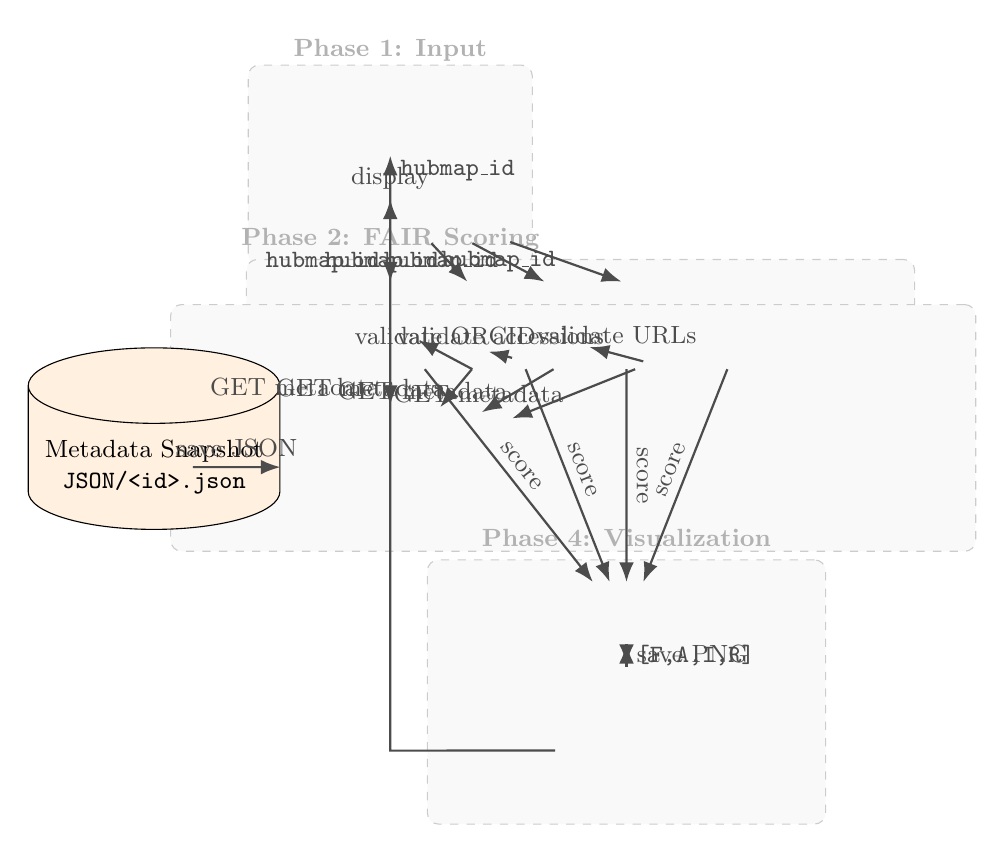
\begin{tikzpicture}[
  node distance=8mm and 15mm,
  font=\small,
  on grid,
  % Node styles
  user/.style={rectangle, rounded corners=3pt, draw=black, fill=blue!12, inner sep=8pt, align=center, minimum width=2.5cm},
  process/.style={rectangle, rounded corners=3pt, draw=black, fill=green!10, inner sep=6pt, align=center, minimum width=2.2cm},
  api/.style={ellipse, draw=black, fill=yellow!15, inner sep=6pt, align=center, minimum width=2cm},
  storage/.style={cylinder, shape border rotate=90, aspect=0.3, draw=black, fill=orange!12, inner sep=6pt, align=center, minimum width=1.8cm},
  phase/.style={rectangle, draw=none, fill=none, inner sep=4pt, font=\bfseries\small, text=gray!60},
  arr/.style={-{Latex[length=2.5mm]}, thick, color=black!70},
  phasebox/.style={rectangle, draw=gray!40, dashed, fill=gray!5, inner sep=8pt, rounded corners=4pt}
]

  % Phase 1: Input
  \node[user] (user) {User\\\texttt{hubmap\_id}};
  \node[process, below=of user] (ui) {Streamlit UI\\\texttt{streamlit\_app.py}};
  
  \begin{scope}[local bounding box=phase1]
    \node[phase, above=of user, yshift=3mm] {Phase 1: Input};
  \end{scope}
  \node[fit=(user)(ui), phasebox] {};

  % Phase 2: Processing - FAIR Modules
  \node[process, below=of ui, yshift=-8mm] (F) {Findable\\\texttt{fair/findable.py}};
  \node[process, right=of F] (A) {Accessible\\\texttt{fair/accessible.py}};
  \node[process, right=of A] (I) {Interoperable\\\texttt{fair/interoperable.py}};
  \node[process, right=of I] (R) {Reproducible\\\texttt{fair/reproducible.py}};
  
  \begin{scope}[local bounding box=phase2]
    \node[phase, above=of F, yshift=3mm] {Phase 2: FAIR Scoring};
  \end{scope}
  \node[fit=(F)(A)(I)(R), phasebox] {};

  % Phase 3: External APIs
  \node[api, below=of F, yshift=-10mm] (entity) {HuBMAP Entity API\\\texttt{/entities/\{id\}}};
  \node[api, below=of A] (orcid) {ORCID API\\\texttt{pub.orcid.org}};
  \node[api, below=of I] (uniprot) {UniProt REST\\\texttt{rest.uniprot.org}};
  \node[api, below=of R] (doi) {DOI Resolvers\\\texttt{doi.org / dx.doi.org}};
  
  \begin{scope}[local bounding box=phase3]
    \node[phase, above=of entity, yshift=3mm] {Phase 3: External Validation};
  \end{scope}
  \node[fit=(entity)(orcid)(uniprot)(doi), phasebox] {};

  % Phase 4: Output
  \node[process, below=of entity, yshift=-12mm, xshift=30mm] (aggregate) {Aggregate Scores\\\texttt{[F, A, I, R]}};
  \node[process, below=of aggregate] (plot) {Plotter\\\texttt{fairhelp.create\_fair\_plot}};
  \node[storage, below=of plot] (png) {PNG File\\\texttt{heatmap}};
  
  \begin{scope}[local bounding box=phase4]
    \node[phase, above=of aggregate, yshift=3mm] {Phase 4: Visualization};
  \end{scope}
  \node[fit=(aggregate)(plot)(png), phasebox] {};

  % Storage (metadata snapshot)
  \node[storage, left=of entity, xshift=-15mm] (jsonmeta) {Metadata Snapshot\\\texttt{JSON/<id>.json}};

  % Edges: Phase 1 → Phase 2
  \draw[arr] (user) -- node[right] {\texttt{hubmap\_id}} (ui);
  
  % Edges: Phase 2 (UI → FAIR modules)
  \draw[arr] (ui) -- node[left] {\texttt{hubmap\_id}} (F);
  \draw[arr] (ui) -- node[left] {\texttt{hubmap\_id}} (A);
  \draw[arr] (ui) -- node[left] {\texttt{hubmap\_id}} (I);
  \draw[arr] (ui) -- node[left] {\texttt{hubmap\_id}} (R);

  % Edges: Phase 2 → Phase 3 (FAIR modules → APIs)
  \draw[arr] (F) -- node[left] {GET metadata} (entity);
  \draw[arr] (A) -- node[left] {GET metadata} (entity);
  \draw[arr] (I) -- node[left] {GET metadata} (entity);
  \draw[arr] (R) -- node[left] {GET metadata} (entity);
  
  \draw[arr] (F) -- node[above] {validate ORCID} (orcid);
  \draw[arr] (F) -- node[above] {validate accessions} (uniprot);
  \draw[arr] (A) -- node[above] {validate URLs} (doi);

  % Edges: Metadata snapshot
  \draw[arr] (entity) -- node[above] {save JSON} (jsonmeta);

  % Edges: Phase 2 → Phase 4 (FAIR modules → Aggregate)
  \draw[arr] (F) -- node[above, sloped] {score} (aggregate);
  \draw[arr] (A) -- node[above, sloped] {score} (aggregate);
  \draw[arr] (I) -- node[above, sloped] {score} (aggregate);
  \draw[arr] (R) -- node[above, sloped] {score} (aggregate);

  % Edges: Phase 4 (Visualization flow)
  \draw[arr] (aggregate) -- node[right] {\texttt{[F,A,I,R]}} (plot);
  \draw[arr] (plot) -- node[right] {save PNG} (png);
  \draw[arr] (png) -- ++(-30mm,0) |- node[pos=0.7, above] {display} (ui);

\end{tikzpicture}
\caption{Live scoring data flow: User enters \texttt{hubmap\_id}, Streamlit UI triggers four FAIR scoring modules in parallel. Each module fetches metadata from HuBMAP Entity API and performs external validations. Scores are aggregated into a 4-element vector, plotted as a 2$\times$2 heatmap, and displayed back to the user. Metadata snapshots are saved locally.}
\label{fig:live_scoring}
\end{figure}


\clearpage
\subsection{Diagram 2: Batch precompute + explore path (\texttt{create\_fair\_json.py} + \texttt{streamlit\_test.py})}
% Improved TikZ diagram for Batch Precompute + Explore Path
% Two-phase layout with clear separation

\begin{figure}[h!]
\centering
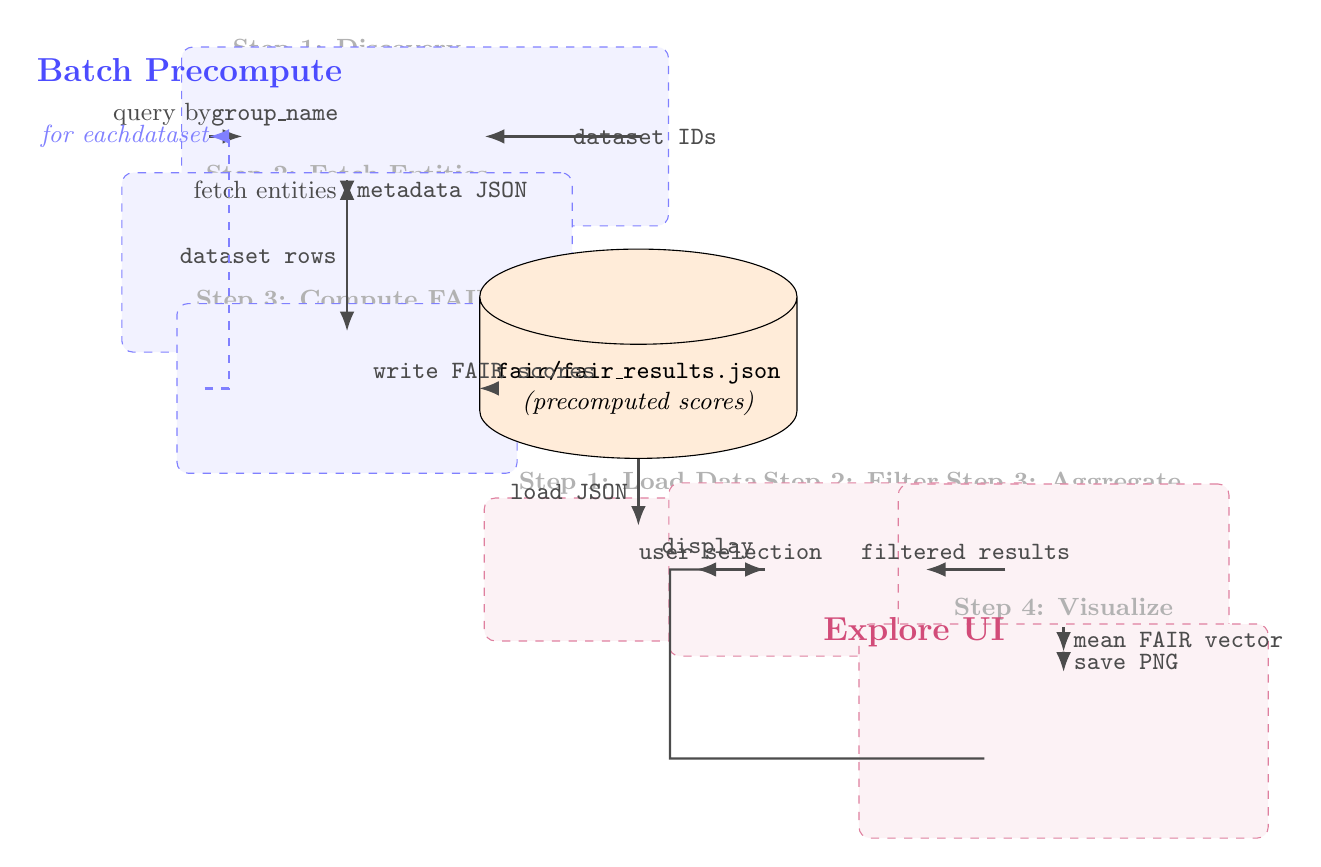
\begin{tikzpicture}[
  node distance=8mm and 12mm,
  font=\small,
  on grid,
  % Node styles
  process/.style={rectangle, rounded corners=3pt, draw=black, fill=green!10, inner sep=6pt, align=center, minimum width=2.2cm},
  api/.style={ellipse, draw=black, fill=yellow!15, inner sep=6pt, align=center, minimum width=2cm},
  storage/.style={cylinder, shape border rotate=90, aspect=0.3, draw=black, fill=orange!15, inner sep=6pt, align=center, minimum width=2cm},
  phase/.style={rectangle, draw=none, fill=none, inner sep=4pt, font=\bfseries\small, text=gray!60},
  arr/.style={-{Latex[length=2.5mm]}, thick, color=black!70},
  phasebox/.style={rectangle, draw=blue!50, dashed, fill=blue!5, inner sep=10pt, rounded corners=4pt},
  phasebox2/.style={rectangle, draw=purple!50, dashed, fill=purple!5, inner sep=10pt, rounded corners=4pt}
]

  % ============================================
  % LEFT SIDE: Batch Precompute Workflow
  % ============================================
  
  % Phase 1: Discovery
  \node[process] (batch) {Batch Builder\\\texttt{create\_fair\_json.py}};
  \node[api, right=of batch] (search) {HuBMAP Search API\\\texttt{hubmap\_sdk}};
  
  \begin{scope}[local bounding box=batch1]
    \node[phase, above=of batch, yshift=3mm] {Step 1: Discovery};
  \end{scope}
  \node[fit=(batch)(search), phasebox] {};

  % Phase 2: Fetch Entities
  \node[api, below=of batch, yshift=-8mm] (entity) {HuBMAP Entity API\\\texttt{/entities/\{id\}}};
  
  \begin{scope}[local bounding box=batch2]
    \node[phase, above=of entity, yshift=3mm] {Step 2: Fetch Entities};
  \end{scope}
  \node[fit=(entity), phasebox] {};

  % Phase 3: Compute FAIR
  \node[process, below=of entity, yshift=-8mm] (score) {Compute FAIR Scores\\\texttt{fair/*.py}\\\texttt{(for each dataset)}};
  
  \begin{scope}[local bounding box=batch3]
    \node[phase, above=of score, yshift=3mm] {Step 3: Compute FAIR};
  \end{scope}
  \node[fit=(score), phasebox] {};

  % Central Storage (connects both workflows)
  \node[storage, right=of score, xshift=25mm] (results) {\texttt{fair/fair\_results.json}\\\textit{(precomputed scores)}};

  % ============================================
  % RIGHT SIDE: Explore UI Workflow
  % ============================================
  
  % Phase 1: Load
  \node[process, below=of results, yshift=-15mm] (ui) {Explore UI\\\texttt{streamlit\_test.py}};
  
  \begin{scope}[local bounding box=explore1]
    \node[phase, above=of ui, yshift=3mm] {Step 1: Load Data};
  \end{scope}
  \node[fit=(ui), phasebox2] {};

  % Phase 2: Filter
  \node[process, right=of ui, xshift=15mm] (filter) {Filter \& Select\\\texttt{fair/utils.py}\\\texttt{(by Lab/Assay/ID/All)}};
  
  \begin{scope}[local bounding box=explore2]
    \node[phase, above=of filter, yshift=3mm] {Step 2: Filter};
  \end{scope}
  \node[fit=(filter), phasebox2] {};

  % Phase 3: Aggregate
  \node[process, right=of filter, xshift=15mm] (agg) {Aggregate\\\texttt{mean\_fair\_results()}\\\texttt{[F, A, I, R]}};
  
  \begin{scope}[local bounding box=explore3]
    \node[phase, above=of agg, yshift=3mm] {Step 3: Aggregate};
  \end{scope}
  \node[fit=(agg), phasebox2] {};

  % Phase 4: Visualize
  \node[process, below=of agg, yshift=-8mm] (plot) {Plotter\\\texttt{fairhelp.create\_fair\_plot}};
  \node[storage, below=of plot] (png) {PNG File\\\texttt{heatmap}};
  
  \begin{scope}[local bounding box=explore4]
    \node[phase, above=of plot, yshift=3mm] {Step 4: Visualize};
  \end{scope}
  \node[fit=(plot)(png), phasebox2] {};

  % ============================================
  % Edges: Batch Precompute Workflow
  % ============================================
  
  % Discovery phase
  \draw[arr] (batch) -- node[above] {query by\\\texttt{group\_name}} (search);
  \draw[arr] (search) -- node[right] {\texttt{dataset IDs}} (batch);
  
  % Fetch phase
  \draw[arr] (batch) -- node[left] {fetch entities} (entity);
  \draw[arr] (entity) -- node[right] {\texttt{metadata JSON}} (batch);
  
  % Compute phase
  \draw[arr] (batch) -- node[left] {\texttt{dataset rows}} (score);
  \draw[arr] (score) -- node[above] {\texttt{write FAIR scores}} (results);
  
  % Iteration indicator
  \draw[arr, dashed, color=blue!50] (score) -- ++(-15mm,0) |- node[pos=0.7, left] {\textit{for each\\dataset}} (batch);

  % ============================================
  % Edges: Explore UI Workflow
  % ============================================
  
  % Load phase
  \draw[arr] (results) -- node[left] {\texttt{load JSON}} (ui);
  
  % Filter phase
  \draw[arr] (ui) -- node[above] {\texttt{user selection}} (filter);
  
  % Aggregate phase
  \draw[arr] (filter) -- node[above] {\texttt{filtered results}} (agg);
  
  % Visualize phase
  \draw[arr] (agg) -- node[right] {\texttt{mean FAIR vector}} (plot);
  \draw[arr] (plot) -- node[right] {\texttt{save PNG}} (png);
  \draw[arr] (png) -- ++(-50mm,0) |- node[pos=0.7, above] {\texttt{display}} (ui);

  % ============================================
  % Labels for workflow separation
  % ============================================
  \node[above=of batch, xshift=-20mm, font=\bfseries\large, text=blue!70] {Batch Precompute};
  \node[below=of ui, xshift=35mm, font=\bfseries\large, text=purple!70] {Explore UI};

\end{tikzpicture}
\caption{Batch precompute + explore workflow: (Left) Batch builder discovers datasets via Search API, fetches entities, computes FAIR scores iteratively, and writes to \texttt{fair/fair\_results.json}. (Right) Explore UI loads precomputed JSON, filters by user criteria (Lab/Assay/ID/All), aggregates mean FAIR scores, and visualizes as a heatmap. The JSON file serves as the bridge between the two workflows.}
\label{fig:batch_explore}
\end{figure}


\subsection{Graphviz Versions}
The same diagrams are also available as Graphviz DOT files for use with external tools:
\begin{itemize}[leftmargin=2em]
  \item \texttt{diagram\_live\_scoring.dot} --- Live scoring workflow
  \item \texttt{diagram\_batch\_explore.dot} --- Batch precompute + explore workflow
\end{itemize}
These can be rendered using Graphviz tools:
\begin{lstlisting}[style=base]
dot -Tpng diagram_live_scoring.dot -o diagram_live_scoring.png
dot -Tpdf diagram_batch_explore.dot -o diagram_batch_explore.pdf
\end{lstlisting}

\section{Operational Notes and Limitations}
\begin{itemize}[leftmargin=2em]
  \item \textbf{Network dependence}: scoring relies on live external API calls; network or service instability affects results.
  \item \textbf{Local side effects}: metadata fetch writes \texttt{JSON/<hubmap\_id>.json}; plotting writes PNG files in the current working directory.
  \item \textbf{Potential score inflation}: some checks return ``pass'' on missing keys or exceptions; this can increase scores for incomplete metadata.
  \item \textbf{Reproducible random trials}: \texttt{\_\_average\_metadata\_success} uses a random number of trials and returns \texttt{int(success\_rate)}; this becomes 1 only when success rate is 100\%.
  \item \textbf{Naming collisions}: in \texttt{streamlit\_app.py}, variables named \texttt{findable}, \texttt{accessible}, etc. overwrite imported function names within scope.
  \item \textbf{Stale/unused dependencies}: \texttt{plotly}, \texttt{seaborn}, and \texttt{humanize} are declared but not clearly exercised by the main execution paths.
\end{itemize}

\section{How to Run (Suggested)}
\subsection{Install dependencies}
\begin{lstlisting}[style=base,caption={Install dependencies.}]
python -m venv .venv
source .venv/bin/activate
pip install -r requirements.txt
\end{lstlisting}

\subsection{Run live scoring app}
\begin{lstlisting}[style=base,caption={Run live scoring Streamlit app.}]
streamlit run streamlit_app.py
\end{lstlisting}

\subsection{(Optional) Precompute batch JSON, then run explore app}
\begin{lstlisting}[style=base,caption={Precompute results then explore.}]
python create_fair_json.py
streamlit run streamlit_test.py
\end{lstlisting}

\appendix
\section{Appendix A: XML Data Flow Diagram (Node/Edge Representation)}
\begin{lstlisting}[style=xml,caption={XML data flow model capturing the system nodes and edges.}]
<dataFlowDiagram name="dont-be-square">
  <nodes>
    <node id="user" label="User" type="actor"/>
    <node id="ui_live" label="Streamlit UI (streamlit_app.py)" type="process"/>
    <node id="ui_explore" label="Streamlit UI (streamlit_test.py)" type="process"/>
    <node id="batch" label="Batch builder (create_fair_json.py)" type="process"/>

    <node id="findable" label="FAIR Findable (fair/findable.py)" type="process"/>
    <node id="accessible" label="FAIR Accessible (fair/accessible.py)" type="process"/>
    <node id="interoperable" label="FAIR Interoperable (fair/interoperable.py)" type="process"/>
    <node id="reproducible" label="FAIR Reproducible (fair/reproducible.py)" type="process"/>

    <node id="hubmap_entity" label="HuBMAP Entity API" type="externalService"/>
    <node id="hubmap_search" label="HuBMAP Search API (via hubmap_sdk)" type="externalService"/>
    <node id="orcid" label="ORCID API" type="externalService"/>
    <node id="uniprot" label="UniProt REST API" type="externalService"/>
    <node id="doi" label="DOI resolvers (doi.org / dx.doi.org)" type="externalService"/>

    <node id="plot" label="Plotter (fairhelp.create_fair_plot)" type="process"/>
    <node id="png" label="PNG heatmap file" type="dataStore"/>
    <node id="json_meta" label="JSON/<hubmap_id>.json" type="dataStore"/>
    <node id="fair_results" label="fair/fair_results.json" type="dataStore"/>
  </nodes>

  <edges>
    <!-- Live path -->
    <edge from="user" to="ui_live" label="enter hubmap_id + click"/>
    <edge from="ui_live" to="findable" label="hubmap_id"/>
    <edge from="ui_live" to="accessible" label="hubmap_id"/>
    <edge from="ui_live" to="interoperable" label="hubmap_id"/>
    <edge from="ui_live" to="reproducible" label="hubmap_id"/>

    <edge from="findable" to="hubmap_entity" label="GET /entities/{id}"/>
    <edge from="accessible" to="hubmap_entity" label="GET /entities/{id}"/>
    <edge from="interoperable" to="hubmap_entity" label="GET /entities/{id}"/>
    <edge from="reproducible" to="hubmap_entity" label="GET /entities/{id}"/>

    <edge from="findable" to="orcid" label="validate contributor/contact ORCID"/>
    <edge from="findable" to="uniprot" label="validate antibody accessions"/>
    <edge from="accessible" to="doi" label="validate DOI URLs"/>

    <edge from="findable" to="json_meta" label="write metadata snapshot"/>
    <edge from="accessible" to="json_meta" label="write metadata snapshot"/>
    <edge from="interoperable" to="json_meta" label="write metadata snapshot"/>
    <edge from="reproducible" to="json_meta" label="write metadata snapshot"/>

    <edge from="ui_live" to="plot" label="FAIR scores (4 floats)"/>
    <edge from="plot" to="png" label="save PNG"/>
    <edge from="png" to="ui_live" label="display image"/>

    <!-- Batch + explore path -->
    <edge from="batch" to="hubmap_search" label="search by group_name"/>
    <edge from="batch" to="hubmap_entity" label="fetch entities by id"/>
    <edge from="batch" to="fair_results" label="write precomputed FAIR arrays"/>
    <edge from="ui_explore" to="fair_results" label="read JSON into DataFrame"/>
    <edge from="ui_explore" to="plot" label="mean FAIR scores"/>
    <edge from="plot" to="png" label="save PNG"/>
    <edge from="png" to="ui_explore" label="display image"/>
  </edges>
</dataFlowDiagram>
\end{lstlisting}

\section{Appendix B: Key code excerpts (for traceability)}
\subsection{Live UI entrypoint (\texttt{streamlit\_app.py})}
\begin{lstlisting}[style=python]
hubmap_id = st.text_input("Enter HuBMAP Dataset ID:", value="HBM666.NDQZ.365")
if st.button("Calculate FAIR Score") and hubmap_id:
    findable = findable(hubmap_id)[0]
    accessible = accessible(hubmap_id)[0]
    interoperable = interoperable(hubmap_id)[0]
    reproducible = reproducible(hubmap_id)[0]
    fair = [findable, accessible, interoperable, reproducible]
    fairhelp.create_fair_plot(np.array(fair).reshape(2, 2), output_file=output_file)
    st.image(output_file)
\end{lstlisting}

\subsection{Metadata fetch (\texttt{fair/findable.py})}
\begin{lstlisting}[style=python]
def __get_metadata(dataset_id: str, api_url: str = "https://entity.api.hubmapconsortium.org/entities") -> Dict:
    response = requests.get(f"{api_url}/{dataset_id}")
    response.raise_for_status()
    metadata = response.json()
    os.makedirs("JSON", exist_ok=True)
    with open(os.path.join("JSON", f"{dataset_id}.json"), "w", encoding="utf-8") as f:
        json.dump(metadata, f, indent=2)
    return metadata
\end{lstlisting}

\end{document}

